\chapter{Background \& Related Works}
\section{Software Defect Prediction}
% 此处需要一张图
In this section, we introduce the related work of software defect prediction. Since machine learning based approach many contain two phase, one is defect metric, another is machine learning model. Figure 4 show the general framework of machine learning base model. 
\begin{figure}
    \centering
    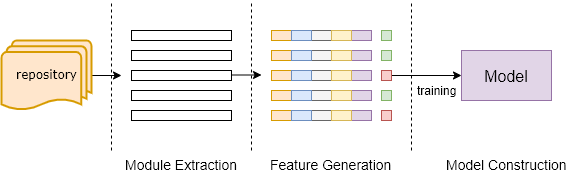
\includegraphics[width=12cm,height=4cm]{pic/defect_overview.png}
    \caption{general framework of machine learning based model}
    \label{fig:my_label}
\end{figure}
\subsubsection{Module Extraction}
To construct a SDP model, the first step we need to extract modules from project, the level can be module, file or function module. Using defect tracking system to label whether each module has bug or not.
\subsubsection{Feature Generation}
The next step is feature generation; after we obtain modules, we need to generate features for each module, their two primary methods to generate feature, one is to apply designed metric to create the feature, another is using deep learning automatically make the feature.
\subsubsection{Model Construction}
After we obtain features and labels of project, i.e dataset, we need to preprocess the dataset so that it can fit the model we selected. Generally, The main problems in the data preprocessing process are data imbalance, data loss and data normalization. Then adopt suitable classification algorithm train a model. Finally, apply the trained model to make other data pretrained 
\subsection{Software Defect Metrics}
There are many forms of metric construction approach, mainly can be divided into three forms of pattern: code-based approach and process-based approach.

\subsubsection{Code-based Approach}
In the early age, Akiyama \cite{} employed \textit{line of code} as metric for SDP. The more code in a file or module, The more likely a file or module have bugs. However, LOC is simple and not enough to indicate the complexity of program. Thereby, in later research, Halstead and MaCabe metric consider the cyclomatic complexity of programs. Halstead metric \cite{} believe that the count of  operand and operator impact program reading speed for reader. The more difficult to read a program, the more possible it contains bug. McCabe metric mainly foucs on control flow of program, if a control flow has higher in this approach. The complexity of the control flow in a program decide whether it has bug or not. However, and the formula is $v(G)=e-n+2$, where $e$ is amount of edge, $n$ is amount of node. In addition, it can calculate the essential complexity and design complexity. With prevalence of OOP, Many researchers begin to design metric for OOP. One of most important metric is CK metric proposed by Chidamber and Kemerer \cite{}. CK metric consider the important of the most coupling, inheritance and cohesion of programs. 

\subsubsection{Process-based Approach}
Software defect are not only associate with code itself, but also associate with external factor. developers' experience and churn of code may result defect problem in software development. 


\section{Deep learning based Software defect Prediction}
With the popularity of NLP development, many researcher begin to apply NLP technique in SDP domain.The advantages of deep learning approach can learn the semantics and syntax of program, which is ignored by traditional model. Such kind of approach show excellent performance compare with traditional machine learning approach.\\

Wang \cite{} extract specific node from AST which was extracted from source code. Then convert these nodes into sequence as input of DBN to generate vector to present semantics of program. After that, they built classification model to by using both defect label and the generated features. The performance of this approach are 14.2\% and 8.9\% higher in F-measurement in terms of WPDP and CPDP,respectively.\\

Encouraged by Wang's approach, Li \cite{} utilize Convolutional neural network to construct the SDP model. They learn from wang's approach, generated semantic featrues by extracting AST nodes from source code. Then the features will be an input of convolutional nerual network. The result show that this approach improved F1 score compared with Wang's.\\

However, such approaches did not consider the level of semantics of program, Dam's el.al \cite{} proposed tree-based LSTM to learn different level semantics of program. They convert different level of node of AST into vector and define a loss function to train node vector to generate vector of AST. Using the AST vector to train SDP model. This approach achieved higher score than existing method in recall.\\

However, when constructing a deep learning model, embedding is necessary for downstream task. The general process is pad the sequence into fixed length. However, if long sequence with more information is condensed into fixed length, it will lose part of information. Thereby, Fan et.al \cite{} propose \textit{BiLSTM}+\textit{attention} method to solve the problem. They first apply \textit{BiLSTM} to extract the semantics feature, then use \textit{attention} to calculate the weight of hidden state generated by \textit{BiLSTM}. The model outperform  state-of-the-art model 14\% and 7\% in F-measure and AUC sorce, respectively. \\

The model that mentioned above have similar problem, i.e without pretrained token vector. Since the defect datasets are small, tokens may not be well-trained and will impact the performance of downstream layer. Thereby, Liang el.al \cite{} pretrained large tokens vector to alleviate this problem. And their proposed model outperform other model both on within-project defect prediction and cross-project defect prediction. \\

\section{Word Emebedding}
In NLP domain, word embedding is based process for downstream task. Since present token through one hot vector may spend large strage, thereby, there are many researches are manage to condense one hot vector into dense vector and present its semantics simulaseously. In this section, we introduce some typical and classic method to embed word.\\

\textbf{Word2Vec}\cite{}, This is typical method that transfer token into vector to present its semantics. In \textit{Word2Vec} model, it is kind of supervisor learning and has two form of model. one is \textbf{skip-gram} and another is \textbf{Continuous-Bag-Of-Word} (CBOW). Skip-gram model is to predict the context tokens when given the center word. and \textbf{CBOW} is the model to predict center token given context. \textit{Word2Vec} is widely apply in NLP task. The aim of \textit{Word2Vec} is to train a word vector that can suit multi task of NLP. However, \textit{Word2Vec} can not handle the problems that tokens in different context present different semantics. \\

\textbf{EMLO} \cite{}. To handle this the problem existed in \textit{Word2Vec}. \textit{EMLO} apply \textbf{BiLSTM} to train a language model. Since it consider double direction of context, it can learn the semantics for identical tokens in different context. 

\textbf{GPT} \cite{}. \textit{GPT} construct from \textit{Transformer} \cite{}. Since \textit{Transformer} can learn the longer distance since that can learn distance context information. Compare with \textit{ELMO}, \textit{GPT} leverage the ability of \textit{Transformer}, can learn longer distance semantics features and it outperform \textit{EMLO} compare with other downstream NLP task.

\textbf{BERT}. \textit{BERT} was proposed by \textit{Google}. \textit{GPT} can only learn one side semantics features. \textit{ELMO} just concatenate bi-direction features generated by \textit{BiLSTM}.  \textit{BERT}\cite{} apply bidirectional \textit{transformer} that truely learn bidirectional context information. In our proposed method, we apply the pretrained \textit{BERT} by using fine tuning to extract the feature. 
